\section{Principes généraux}

\begin{frame}
	\begin{block}{Communication}
		\begin{itemize}
			\item{Entre 2 organismes}
			\item{Modification de l'action del'autre}
			\item{Transmission d'unformation}
			\item{Action indirecte}
		\end{itemize}
	\end{block}
\end{frame}

\begin{frame}
	\begin{block}{Schéma de \textbf{Laswell} (1948)}
		\begin{itemize}
			\item{Qui ?}
			\item{Dit quoi ?}
			\item{Par quel moyen}
			\item{A qui ?}
			\item{Avec quel effet ?}
		\end{itemize}
	\end{block} \pause

	\begin{block}{Schéma de \textbf{Laswell} (1948)}
		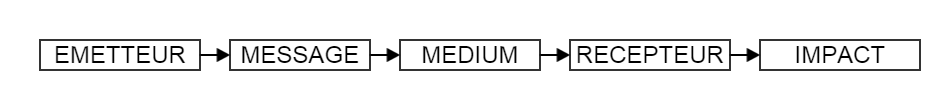
\includegraphics[width=12cm]{laswell.png}
		\begin{itemize}
			\item{Emetteur : source de l'émission}
			\item{Message : ce qui apporte l'information}
			\item{Récepteur : celui qui reçoit le message}
		\end{itemize}
	\end{block}
\end{frame}

\begin{frame}
	\begin{block}{Shannon (1949)}
		\textbf{Théorie de l'information} 
		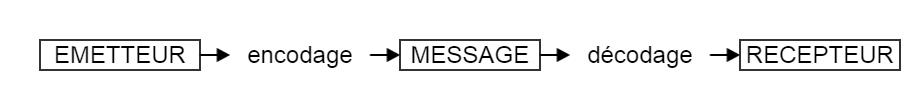
\includegraphics[width=12cm]{shannon.png}
		\begin{itemize}
			\item{Codage : transmission de l'information suivant un système de règles}
			\item{Décodage : lors de la réception de l'information}
			\item{Canal : voie de circulation des messages}
		\end{itemize}
	\end{block}
\end{frame}

\begin{frame}
	\begin{block}{Wiener (1949)}
		\textbf{Régulation : le feed back} 
		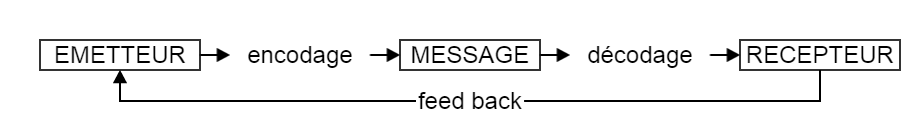
\includegraphics[width=12cm]{wiener.png}
		\begin{itemize}
			\item{Feed back : information de retour. Influe sur l'emetteur qui réajuste donc le message}
			\item{Bruits : ce qui dénature le message}
			\item{Référent : situation et contexte qui amènent à formuler le message}
		\end{itemize}
	\end{block}
\end{frame}
